\chapter{New Roles for Generative AI Co-Creators: Two Case Studies in New Media Public Art Installations}

\subsection{Link to thesis}
This last chapter presents two case studies exploring the potential of human-AI co-creativity in new media practice and public art generative installations. It is organised in two parts.

The first installation was commissioned by the School of Cybernetics at the Australian National University for their public exhibition: “Australian Cybernetics: a point through time”. A corresponding paper was presented at the 11th International Conference on Artificial Intelligence in Music, Sound, Art and Design (EvoMUSART) 2022 conference in Brno, Czech Republic.

The second installation was commissioned by the Sydney Opera House as part of their 50th anniversary celebrations, and a corresponding paper was presented at the Sound and Music Computing (SMC) Conference 2024 in Porto, Portugal.

Both installations were done in collaboration with music studio Uncanny Valley, and they explored the possibility of a new co-creative role for generative AI, particularly an LLM, in the context of data sonification. Specifically, the AI assumed the role of a semantic interpreter of semi-structured data corresponding to the surrounding environment where the installations were presented, and then translated this into an evolving audiovisual soundscape by controlling a music engine. Put simply: translating data from the environment into music in a creatively agentic way.

The core questions guiding the enquiry were: can generative technologies enable new forms of creative practice by assuming novel roles? How well can they fulfil these roles and what are the challenges involved in this type of creative practice? How can this inform my research questions relating to interaction design for effective co-creativity, human agency, assumed roles and dialogic interaction?

\subsection{New roles, new possibilities}

On one hand, experimental creative practice is a valuable research tool in interaction design \cite{Candy2019-vg, Vear2021-cx} and creative technology \cite{Colton2012-jc, Cohen1995-wt, Cope2000-cq, Reichardt1968-eo}. While generative AI presents the possibility to automate existing creative productions, both as an interaction designer and as a creative technologist, I am more interested in exploring its potential for enabling new creative possibilities. I believe this is where most of the co-creative potential between humans and AI lies. An emerging practice is increasingly exploring similar possibilities, as illustrated within the communities of practice in the venues in which this work has been presented, such as SMC and EvoMUSART. This work serves as a further invitation for interaction designers and designers of co-creative systems working with generative AI to explore what latent capabilities exist in these models, what new types of creative practice they can enable, and what novel roles these systems can play.

In this case, I wanted to explore how a generative system, by virtue of turning complex data into a more digestible format (music) could serve as an interface with complex systems. This does not assume the need for a direct translation, as exists in the realm of data visualisation, but rather one that can draw the attention of the audience to the surrounding environment—be it a building, the weather, economic activity or atmospheric phenomena—through its interpretation as a soundscape. Importantly: I explored the possibility of doing so in a semantically rich way, in contrast with sonification approaches that directly map values of the data to sonic qualities. 

\subsection{Generative variability, control and dialogue}

On a practical level, this installation illuminates challenges that have been echoed throughout this thesis and that are reinforced in the conclusion: the challenge of generative variability, where it is difficult to anticipate and predict what the model will do. In some cases, this merely involves the case of fixating on an output over and over, as described in the first paper, or the more visible case of outputting offensive material, as happened during one of the installations.

Addressing this in real time was challenging. Given that the model only worked by executing a generative task based on a system prompt, strategies were constrained to examining logs of inputs and outputs and tweaking the prompt accordingly in a limited attempt to steer future behaviour. This illuminates a potential opportunity for dialogic interaction. One can imagine a dialogic backdoor: a conversational interface where I could steer the model and ask, “why did you make this choice?” or suggest, “you have fixated on that particular element too much, try something different”.

\subsection{Context-awareness for situated co-creativity}


These installations also revealed the capacity for language models to bring in external context. And with this, create artworks that are socially situated. In theory, if the installations were presented elsewhere, the artwork would be different. Of course, this is the case simply because the outputs are ever changing, but it is the hope that the outputs at least would reveal some aspects of the environment they are surrounded by. For example, in the case of the Opera House installation, it was noticeable in the music when the building was empty late at night: the music was mostly calm. In contrast, during peak hours where there was considerable activity in the building, the soundscape became more energetic, sonically crowded and heavy.

Such interactions highlight an aspect I discuss as a part of dialogic interaction: context awareness. Regardless of the particular use case, bringing in the context offers new possibilities for more situated human-AI interactions.

\subsection{Agency}

Lastly, these installations also illuminate a crucial thread throughout my thesis: that of human agency, and the role we played in it. The soundscape produced in these installations was generated using a music engine that arranged, combinatorially, a set of human-made or human-curated music stems. The LLM controlled this engine through selecting some settings, based on interpretations of how best to map the data into the music (the details are provided in the papers).

As such, it can be argued that we, the team, maintained agency over the sonic quality of the outputs, maintaining involvement at the artefact level. Moreover, we constrained the possibilities of how sounds could be combined, to maintain compositional control and intent. This can be understood as a meta-composition, not directly composing the soundscapes but creating the building blocks and providing the constraints within which the AI operated. We engaged the creativity of the AI, in turn, to operate within these bounds and decide how the incoming data would be mapped to soundscapes. I believe this illustrates a promising possibility for human-AI co-creativity: that of ever-evolving pieces, in music, narrative or otherwise, where the human meta-composes, and the AI executes generatively.

Existing generative practices have explored this role of the “human as a gardener”. For example, Brian Eno’s generative practice based on applications of simple rules in music looping. But generative AI opens a possibility where more agency is handed to the AI to make decisions. It also affords the possibility of “talking to the system”—setting goals, aligning meaning—in contrast to previous generative practices where the generative system was a blind compounding of rules that afforded no natural language interaction.

Lastly, to clarify my involvement: I originally developed the approach of semantic sonification described here, and was in charge of the development and implementation for the generative AI, collecting the real-time data and feeding it to the AI components. Uncanny Valley was involved in the development of the music engine that the LLM connected to and controlled.

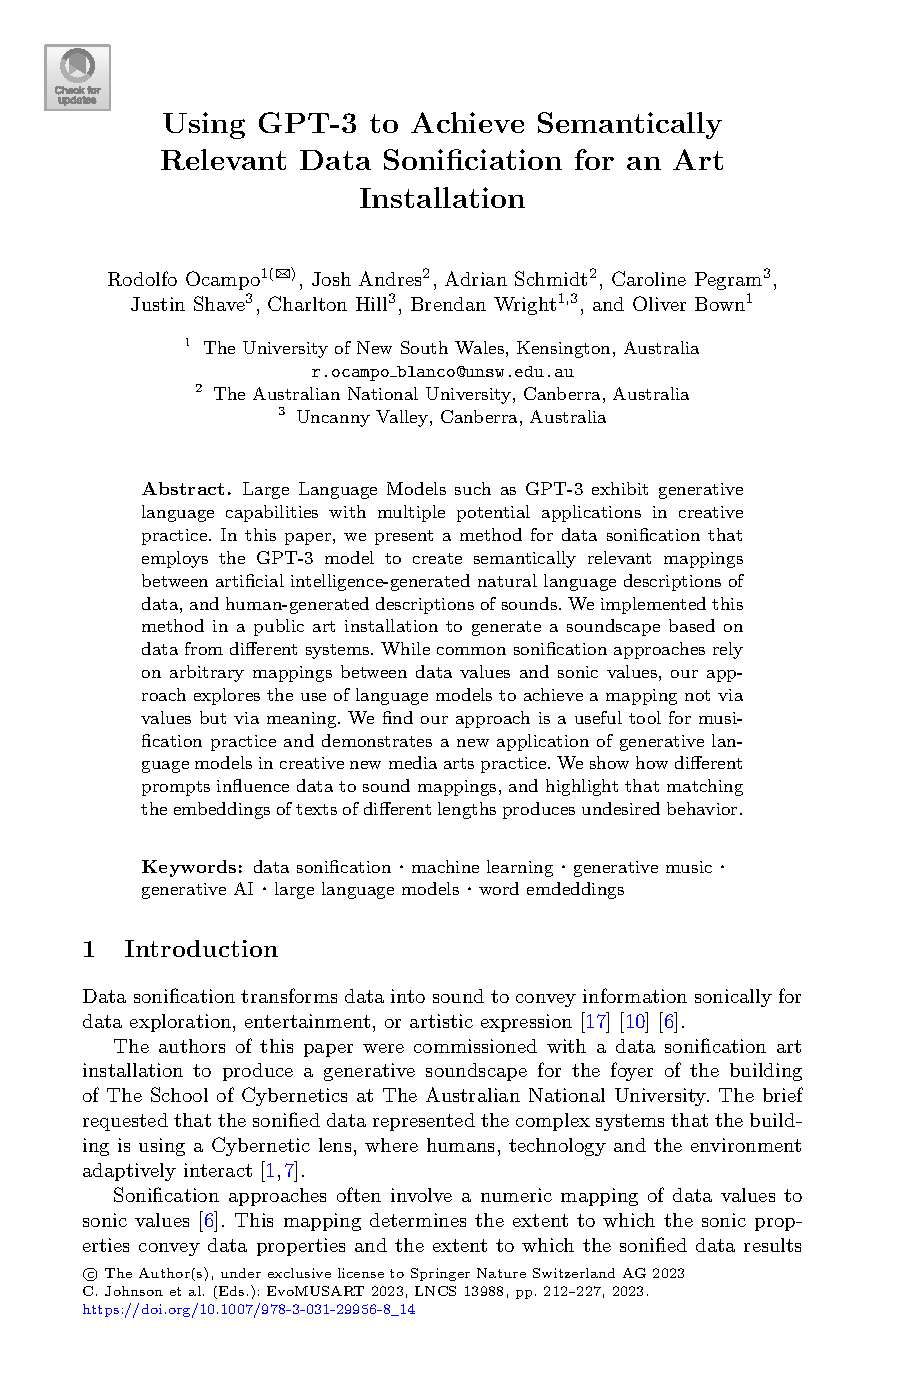
\includepdf[pages=-]{6-techchapter/EvoMusArtPaper.pdf}

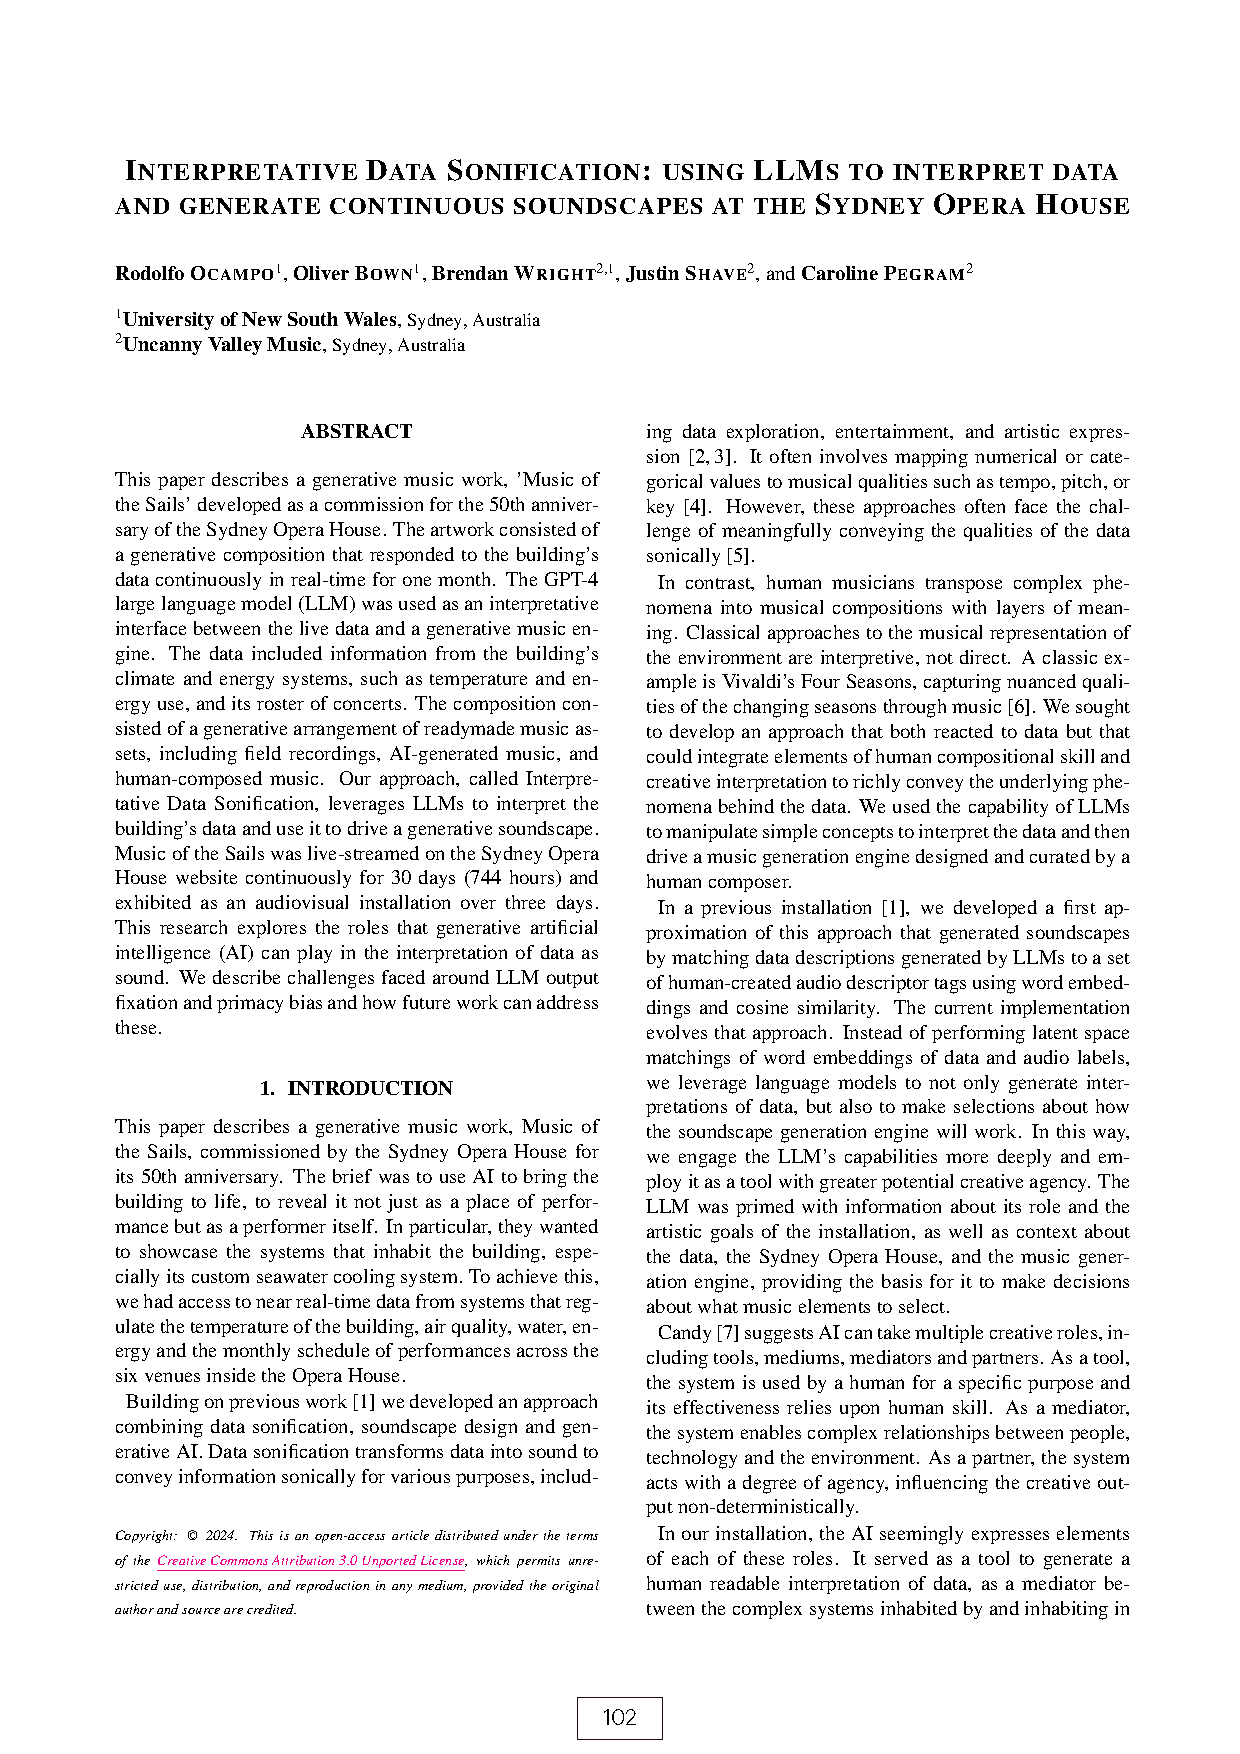
\includepdf[pages=-]{6-techchapter/SMCPaper.pdf}



